\documentclass[a4paper, twocolumn]{article}
\usepackage[pdftex, hidelinks,
            pdftitle={Report},
            pdfauthor={Erik S. Vasconcelos Jansson},
            pdfsubject={Report},
            pdfkeywords={report}]{hyperref}

\usepackage{bm}
\usepackage[T1]{fontenc}
\usepackage[utf8]{inputenc}
\usepackage{algorithmic}
\usepackage{algorithm}
\usepackage{amsfonts}
\usepackage{booktabs}
\usepackage{amssymb}
\usepackage{courier}
\usepackage{booktabs}
\usepackage{graphicx}
\usepackage{listings}
\usepackage{mathtools}
\lstset{basicstyle=\footnotesize\ttfamily,
        breakatwhitespace = false,
        breaklines = true,
        keepspaces = true,
        language = C++,
        showspaces = false,
        showstringspaces = false,
        belowcaptionskip = \bigskipamount,
        framerule = 0.80pt,
        frame = tb,
        numbers = left,
        belowskip = \bigskipamount,
        escapeinside={<@}{@>}}

\title{Introduction to Machine Learning \\
       Individual Laboration Report --2--}
\author{{Erik Sven Vasconcelos Jansson} \\
        {\href{mailto:erija578@student.liu.se}
        {\texttt{erija578@student.liu.se}}} \\
        {Linköping University, \, Sweden}}

\begin{document}
    \pagenumbering{arabic}
    \maketitle % Titles...

    \section*{Assignment 1}

    Reducing the amount of relevant features by using \emph{feature selection} is an important task in \emph{supervised machine learning}. Since many features $\mathcal{F}_i$ are more relevant than others, producing the optimal feature set $\mathcal{\hat{F}} \subseteq \mathcal{F}$, reducing $|\mathcal{F}|$, while also $\hat{\varepsilon}(\mathbf{\hat{y}}, \mathbf{y})$, the \emph{Mean Squared Error (M.S.E)}. Here, we build a \emph{brute-force feature selection} for \emph{linear models}, using \emph{k-folds cross validation} for ranking feature subsets.

    First, every possible feature combination $\mathcal{F}_i \subseteq \mathcal{F}$ is generated. Thereafter, each $\mathcal{F}_i$ is tested through \emph{k-fold cross-validation}, giving the \emph{mean $\hat{\varepsilon}_i(\mathbf{\hat{y}}, \mathbf{y})$} of the feature subset $\mathcal{F}_i$. By picking the feature subset $\mathcal{F}_i$ which produces $\mathrm{min}_i\; \hat{\varepsilon}_i(\mathbf{\hat{y}}, \mathbf{y})$, the best features are picked. In Listing~\ref{lst:featsel} line \texttt{26} we generate all $\mathcal{F}_i$, which are then cross-validated in lines \texttt{30-31}, then in lines \texttt{34-43} the best feature subset $\hat{\mathcal{F}}$ is given by evaluating the errors $\mathrm{min}_i\; \hat{\varepsilon}_i(\mathbf{\hat{y}}, \mathbf{y})$, where $\hat{\mathcal{F}} = \mathcal{F}_i$.

    Now, how \emph{k-fold cross validation} works is shown. Roughly, Algorithm~\ref{alg:kfoldcv} demonstrates these steps, by giving each individual $\mathcal{F}_i$ and respective $X_{\mathcal{F}_i}$, $\mathbf{y}_{\mathcal{F}_i}$ as arguments, the \emph{feature matrix} and \emph{target vector}. For each $\mathcal{F}_i$ and \emph{k-fold iteration}, a \emph{linear hypothesis function} is trained, predicting $\hat{\mathbf{y}}$ using Equations~\ref{eq:linrhat}. Thereafter, the \emph{M.S.E} of the prediction $\hat{\varepsilon}_i(\mathbf{\hat{y}}, \mathbf{y})$, is calculated by using Equation~\ref{eq:mse}. Finally, the \emph{mean} of these $\hat{\varepsilon}_i(\mathbf{\hat{y}}, \mathbf{y})$ is the result of $\mathcal{F}_i$ cross-validation.

    \begin{gather} \label{eq:linrhat}
        \mathbf{\hat{w}}^{}_t = (X_t^\intercal X^{}_t)^{-1} X_t^\intercal \mathbf{y}^{}_t \\
        \mathbf{\hat{y}}^{}_v = X^{}_v \mathbf{\hat{w}}^{}_t
    \end{gather}

    \begin{equation} \label{eq:mse}
        \hat{\varepsilon}(\mathbf{\hat{y}}, \mathbf{y}) = \frac{1}{n}\sum_{i=1}^{n}(\hat{y}_i - y_i)^2
    \end{equation}

    \begin{algorithm}
        \caption{K-Fold Cross-Validation (Linear $\mathcal{M}$)}
    \label{alg:kfoldcv}
    \begin{algorithmic}[1]
        \REQUIRE feature matrix $X_\mathcal{F}$ and target vector $\mathbf{y_\mathcal{F}}$,
                 given a feature selection $\mathcal{F}$ with cardinality $|\mathcal{F}|$.

        \STATE $(X_i, \mathbf{y}_i) \leftarrow \mathrm{split}(X_\mathcal{F}, \mathbf{y}_\mathcal{F}, k)$ \COMMENT{Equally $|X_\mathcal{F}| \div k$}

        \FOR[Attempts every of $k$-folds]{$i \leftarrow 1$ \TO $k$}
            \STATE $X_t \leftarrow X_1 \cup \dots \cup X_k - X_i$ \COMMENT{Except fold $i$}
            \STATE $\mathbf{y}_t \leftarrow \mathbf{y}_1 \cup \dots \cup \mathbf{y}_k - \mathbf{y}_i$ \COMMENT{Except fold $i$}
            \STATE $\mathbf{\hat{w}}_t \leftarrow (X_t^\intercal X^{}_t)^{-1} X_t^\intercal \mathbf{y}^{}_t$ \COMMENT{Train model}
            \STATE $\mathbf{\hat{y}}^{}_i \leftarrow X^{}_i \mathbf{\hat{w}}^{}_t$ \COMMENT{Predict target vector}
            \STATE $\hat{\varepsilon}_i(\mathbf{\hat{y}}_i, \mathbf{y}_i) \leftarrow \frac{1}{n}\sum_{j=1}^{n}(\hat{y}_j - y_j)^2$
        \ENDFOR

        \RETURN $(\sum_{i=1}^k{\hat{\varepsilon}_i(\mathbf{\hat{y}}_i, \mathbf{y}_i)}) \div k$
    \end{algorithmic}
    \end{algorithm}

    The implementation of \emph{feature selection} is found under Listing~\ref{lst:featsel}, while \emph{k-fold cross-validation} should be found in Listing~\ref{lst:kfoldcv}, \emph{linear regression} in Listing~\ref{lst:linrhat}. Most information was derived from \emph{Andrew Ng's Regularization \& Model Selection Handouts}~\cite{ng2016notes}.

    Finally, testing the \emph{swiss dataset} on our \emph{feature selection} implementation where $\mathcal{F} = \mathcal{U} - \mathrm{Fertility}$, gives $\hat{\mathcal{F}} = \{3, 4, 5\}$, also shown in the Table~\ref{table:featsel} below. Our $\hat{\mathcal{F}}$ seems reasonable, being \emph{Catholic} is usually attributed with \emph{low abortion rate}, \emph{Infant Mortality} is directly linearly related as can be seen in the plot.

    \begin{table}[h!]
    \begin{center}
    \begin{tabular}{lc}
        \toprule
            \textbf{Feature Selection} & \textbf{M.S.E.} \\
        \midrule
            $\{3, 4, 5\}$ & $90.6202$ \\
            $\{1, 3, 4, 5\}$ & $111.411$ \\
            $\{1, 2, 3, 5\}$ & $117.092$ \\
        \bottomrule
    \end{tabular}
    \end{center}
    \caption{where 1 $\rightarrow$ \emph{Agriculture}, 2 $\rightarrow$ \emph{Examination}, 3 $\rightarrow$ \emph{Education}, 4 $\rightarrow$ \emph{Catholic}, 5 $\rightarrow$ \emph{Infant Mortality}.}
    \label{table:featsel}
    \end{table}

    \begin{figure}[h!]
        \centering
        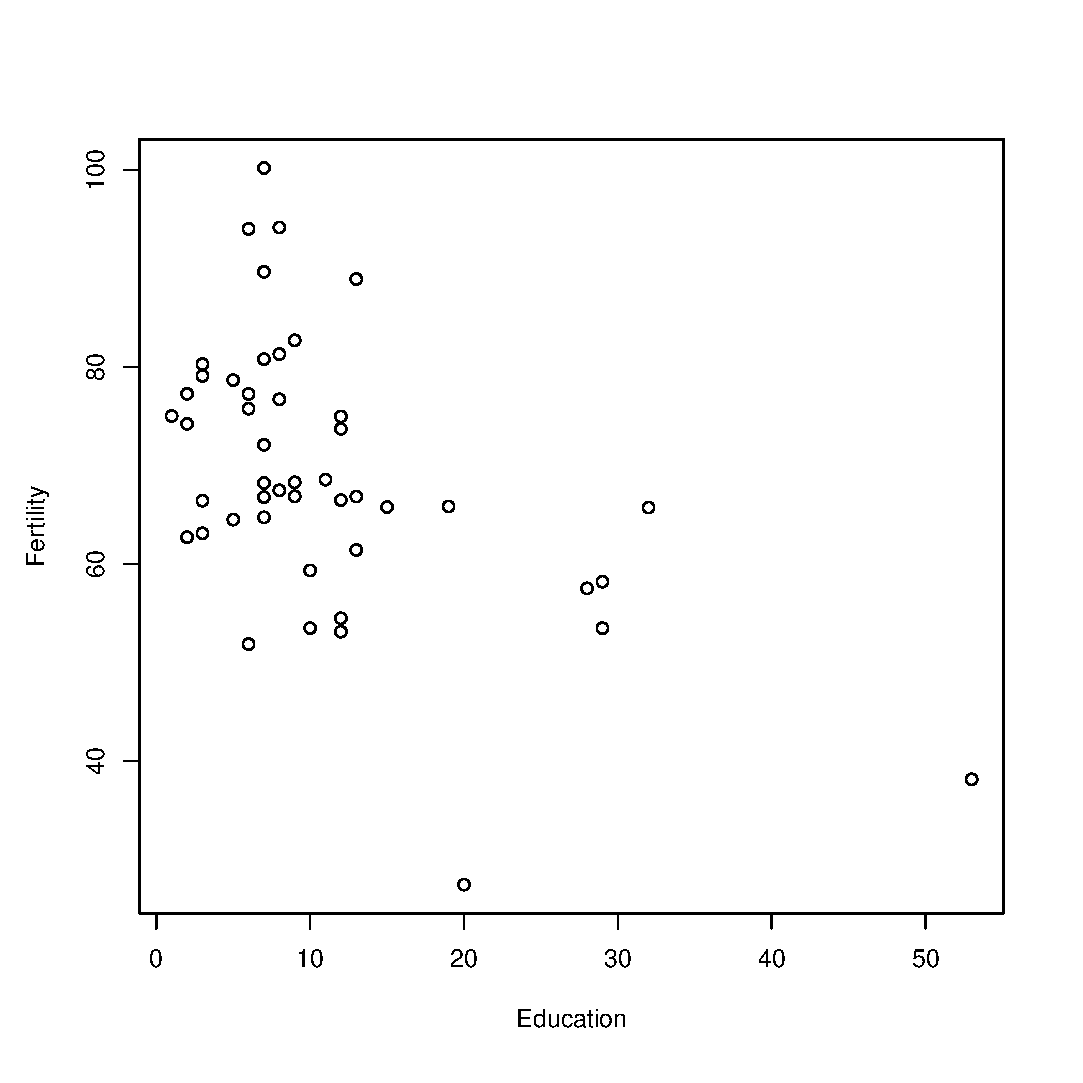
\includegraphics[width=0.26\textwidth]{share/education.eps}
        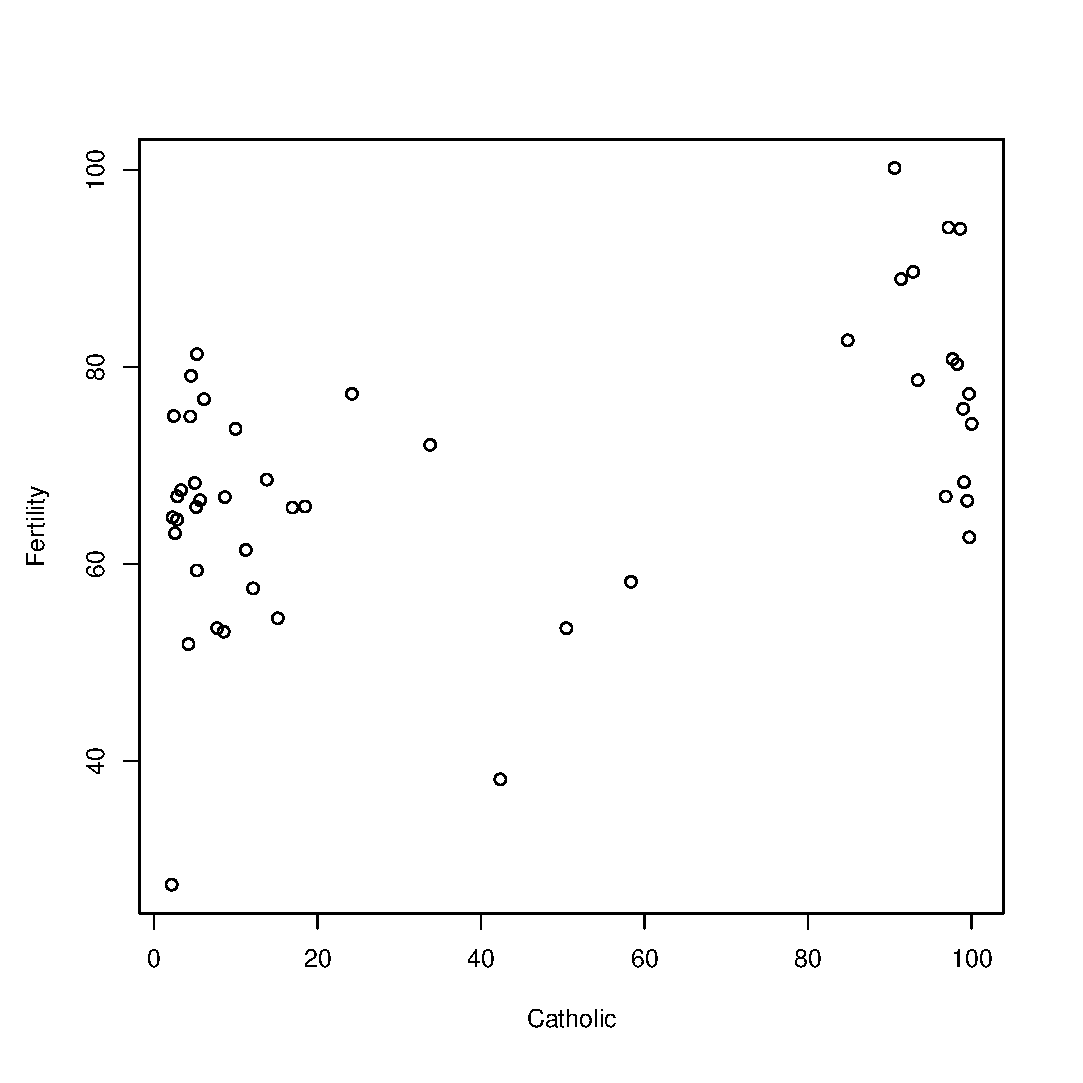
\includegraphics[width=0.26\textwidth]{share/catholic.eps}
        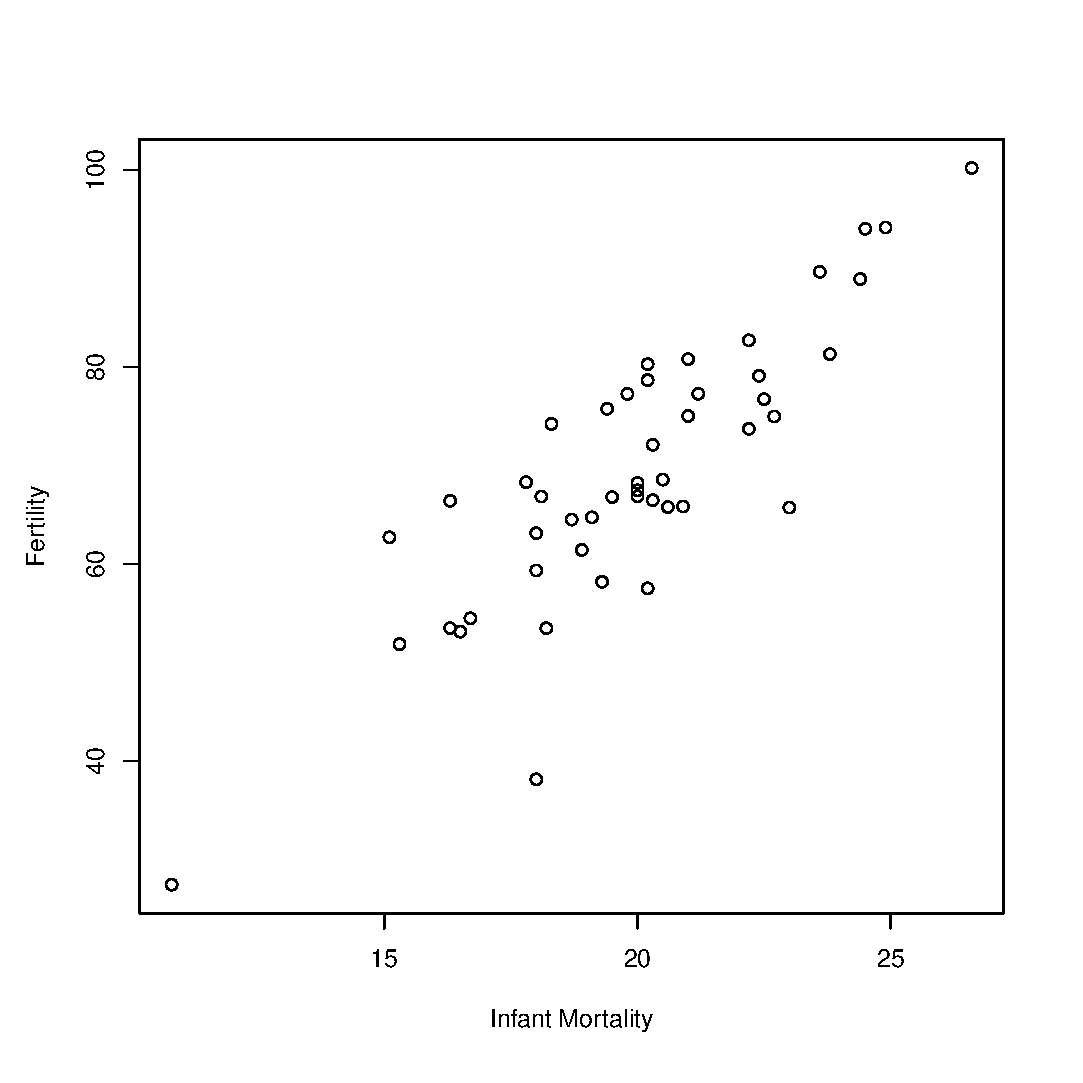
\includegraphics[width=0.26\textwidth]{share/mortality.eps}
    \end{figure}

    \begin{figure}[h!]
        \centering
        \label{fig:kvsmse}
        \caption{displays the relationships between feature subsets of \emph{Size K} and their \emph{Average $M.S.E$}. Notice that the \emph{expected error decreases} by \emph{increases in k}.}
        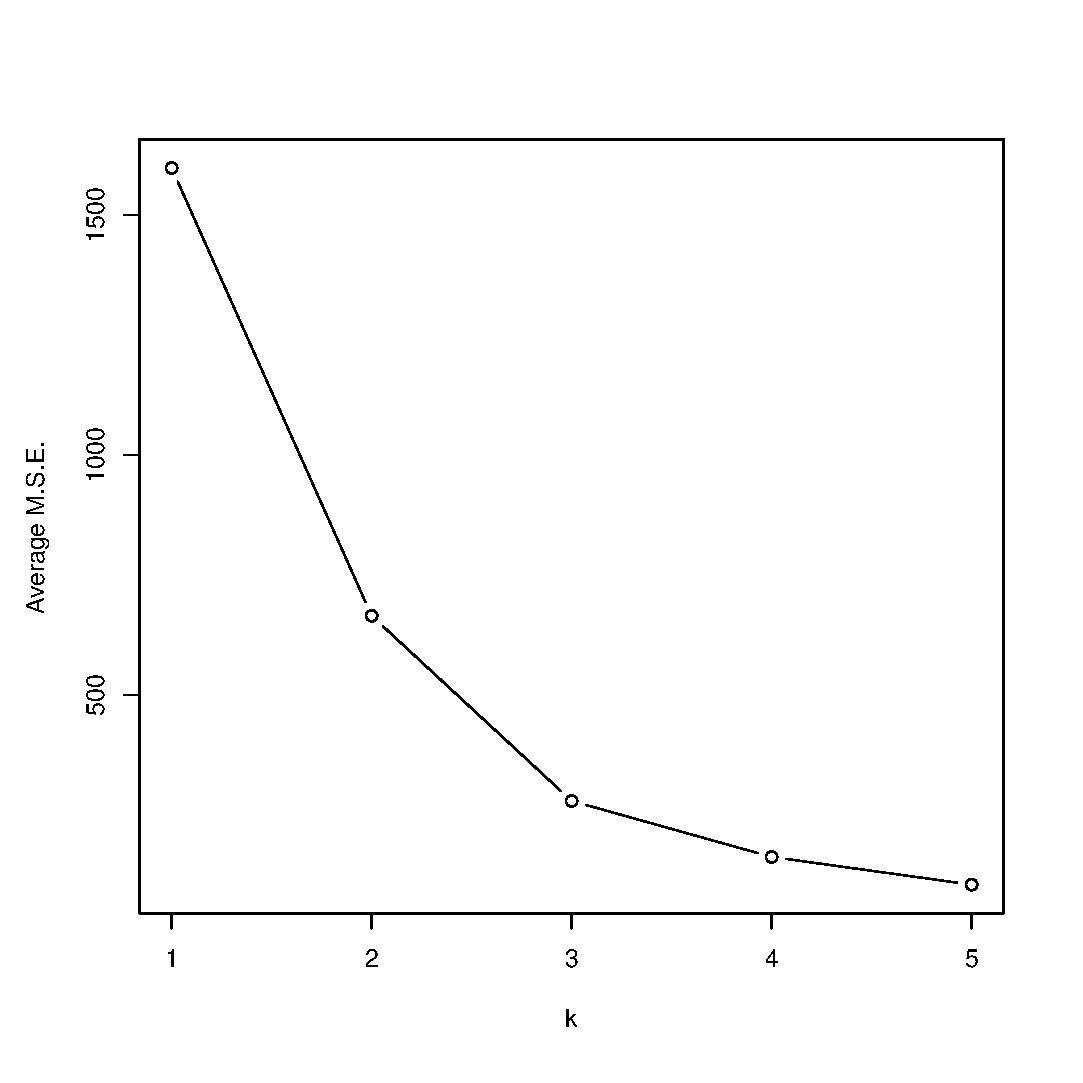
\includegraphics[width=0.36\textwidth]
        {share/kvsmse.eps}
    \end{figure}

    \newpage

    \section*{Assignment 2}

    By using the \emph{tecator dataset}, produced from observations on \emph{predicting fat content} simply by using an \emph{infrared absorbance spectrum} (w.\ several channels), we try to find relationships between their features.

    \begin{figure}[h!]
        \centering
        \caption{relationship seems very close to linear. \emph{Protein} and \emph{Moisture} seem to be related somehow, at least in the provided meat observation datasets.}
        \label{fig:linear}
        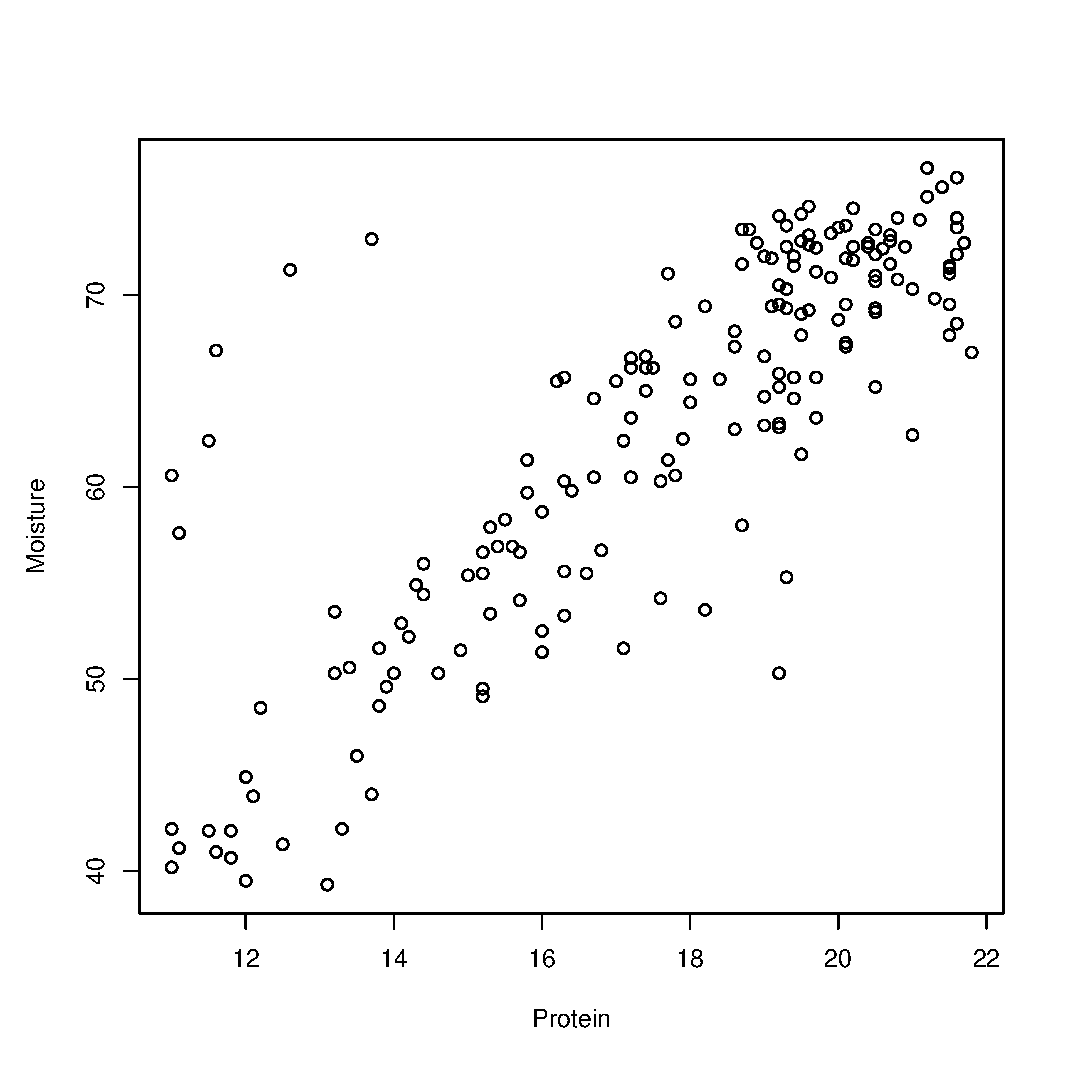
\includegraphics[width=0.32\textwidth]
        {share/linear.eps}
    \end{figure}

    Now we consider models $M_i$ where \emph{Moisture} is \emph{normally distributed} and related to \emph{Protein} with a \emph{polynomial function} of steadily increasing degree. Equation~\ref{eq:poly} displays this relation, MSE in Figure~\ref{fig:depends}.

    \begin{equation} \label{eq:poly}
        \mathrm{Moisture} \sim \mathcal{N}(w_0 + \sum_{i=1}^6{(w_i^i \cdot \mathrm{Protein}_i)}, \sigma^2)
    \end{equation}

    \begin{figure}[h!]
        \centering
        \caption{increasing complexity for the \emph{$i^{th}$ Model} seems to generate \emph{bias} towards the \emph{training dataset}, motivating the higher \emph{validation dataset} error rate.}
        \label{fig:depends}
        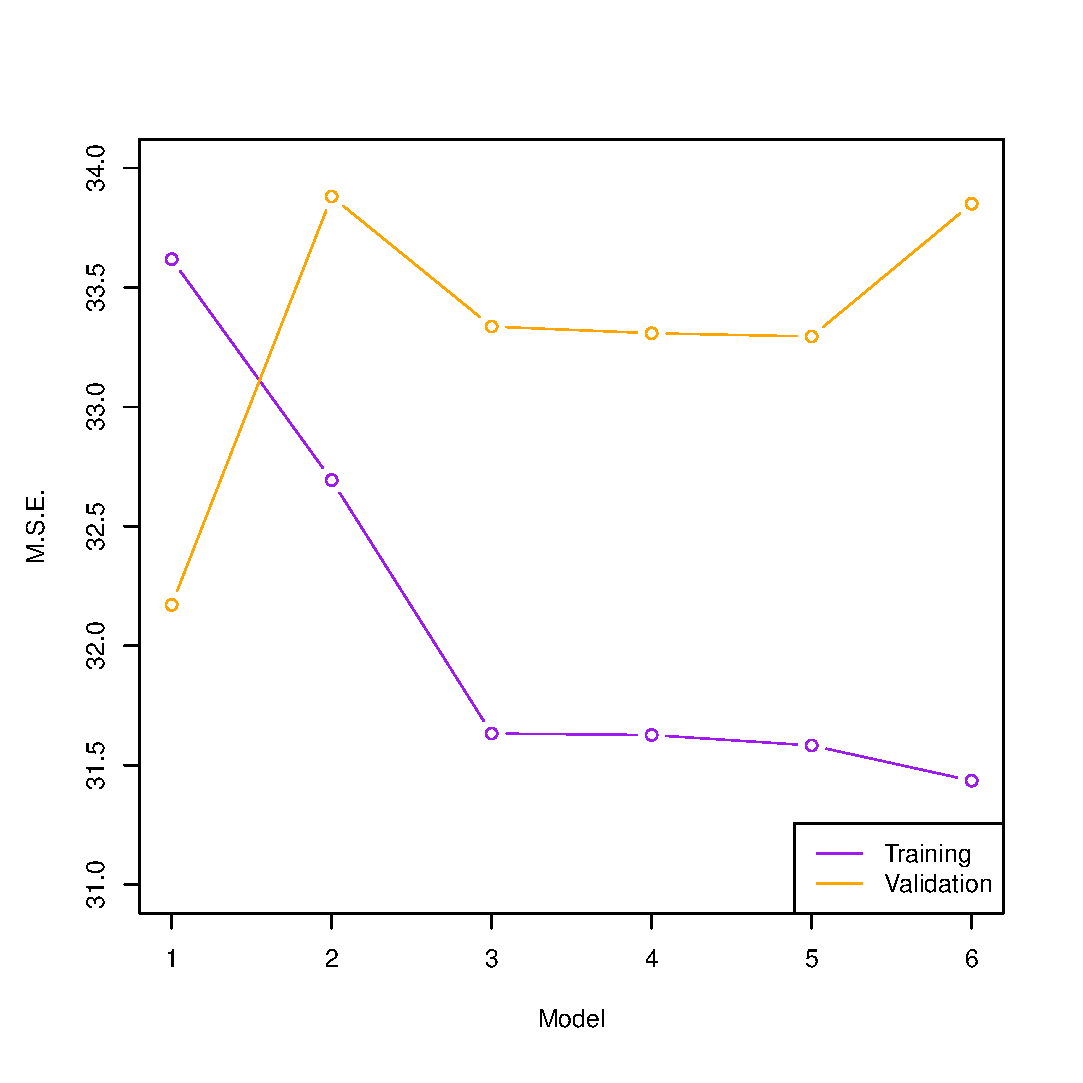
\includegraphics[width=0.32\textwidth]
        {share/depends.eps}
    \end{figure}

    \newpage

    It seems the model \emph{overfits} with more \emph{complexity}. The models $M_i$ and their \emph{M.S.E.}\ are calculated in lines \texttt{24-39} in Listing~\ref{lst:script}, the assignment 2 scripts. Also, according to the plot, the best model $M_i$ is located somewhere between $i = 1$ and $2$, where the lines intersect, producing the lowest M.S.E.\ for \emph{both datasets}, meaning there isn't \emph{bias} towards either $D$.

    Now we perform \emph{feature/variable selection} on the \emph{features Channel1-100} and \emph{target/response} of \emph{Fat}. By using \emph{stepAIC} on a linear model generated with \emph{R's lm}, a total of \emph{64 variables} were selected here. This is done in lines \texttt{66-67} in Listing~\ref{lst:script} (\emph{w.\ MASS}).

    By using the \emph{Ridge regression model} on the same \emph{features} and \emph{response variables} with \emph{glmnet library}. Figure~\ref{fig:lasso_ridge} shows how \emph{coefficients} relate to the \emph{log $\lambda$}, \emph{the log penalty}. Notice how all coefficients \emph{converge uniformly} as \emph{higher penalty} is added to the model. This is being done in line \texttt{72} with $\lambda = 0.0$ (Ridge).

    Thereafter, we use the \emph{LASSO regression model} with the same \emph{features and response variables}. See in Figure~\ref{fig:lasso_ridge} how the \emph{coefficients} converge \emph{iteratively} instead of \emph{simultaneously}, comparing toward \emph{Ridge}. This can be explained graphically within Figure~\ref{fig:shape}.

    \begin{figure}[h!]
        \centering
        \caption{on the left we have \emph{Lasso} and right \emph{Ridge}. Notice, that \emph{Lasso} can set $w_1$ $\rightarrow$ zero much faster. Distributed under CC by Rezamohammadighazi.}
        \label{fig:shape}
        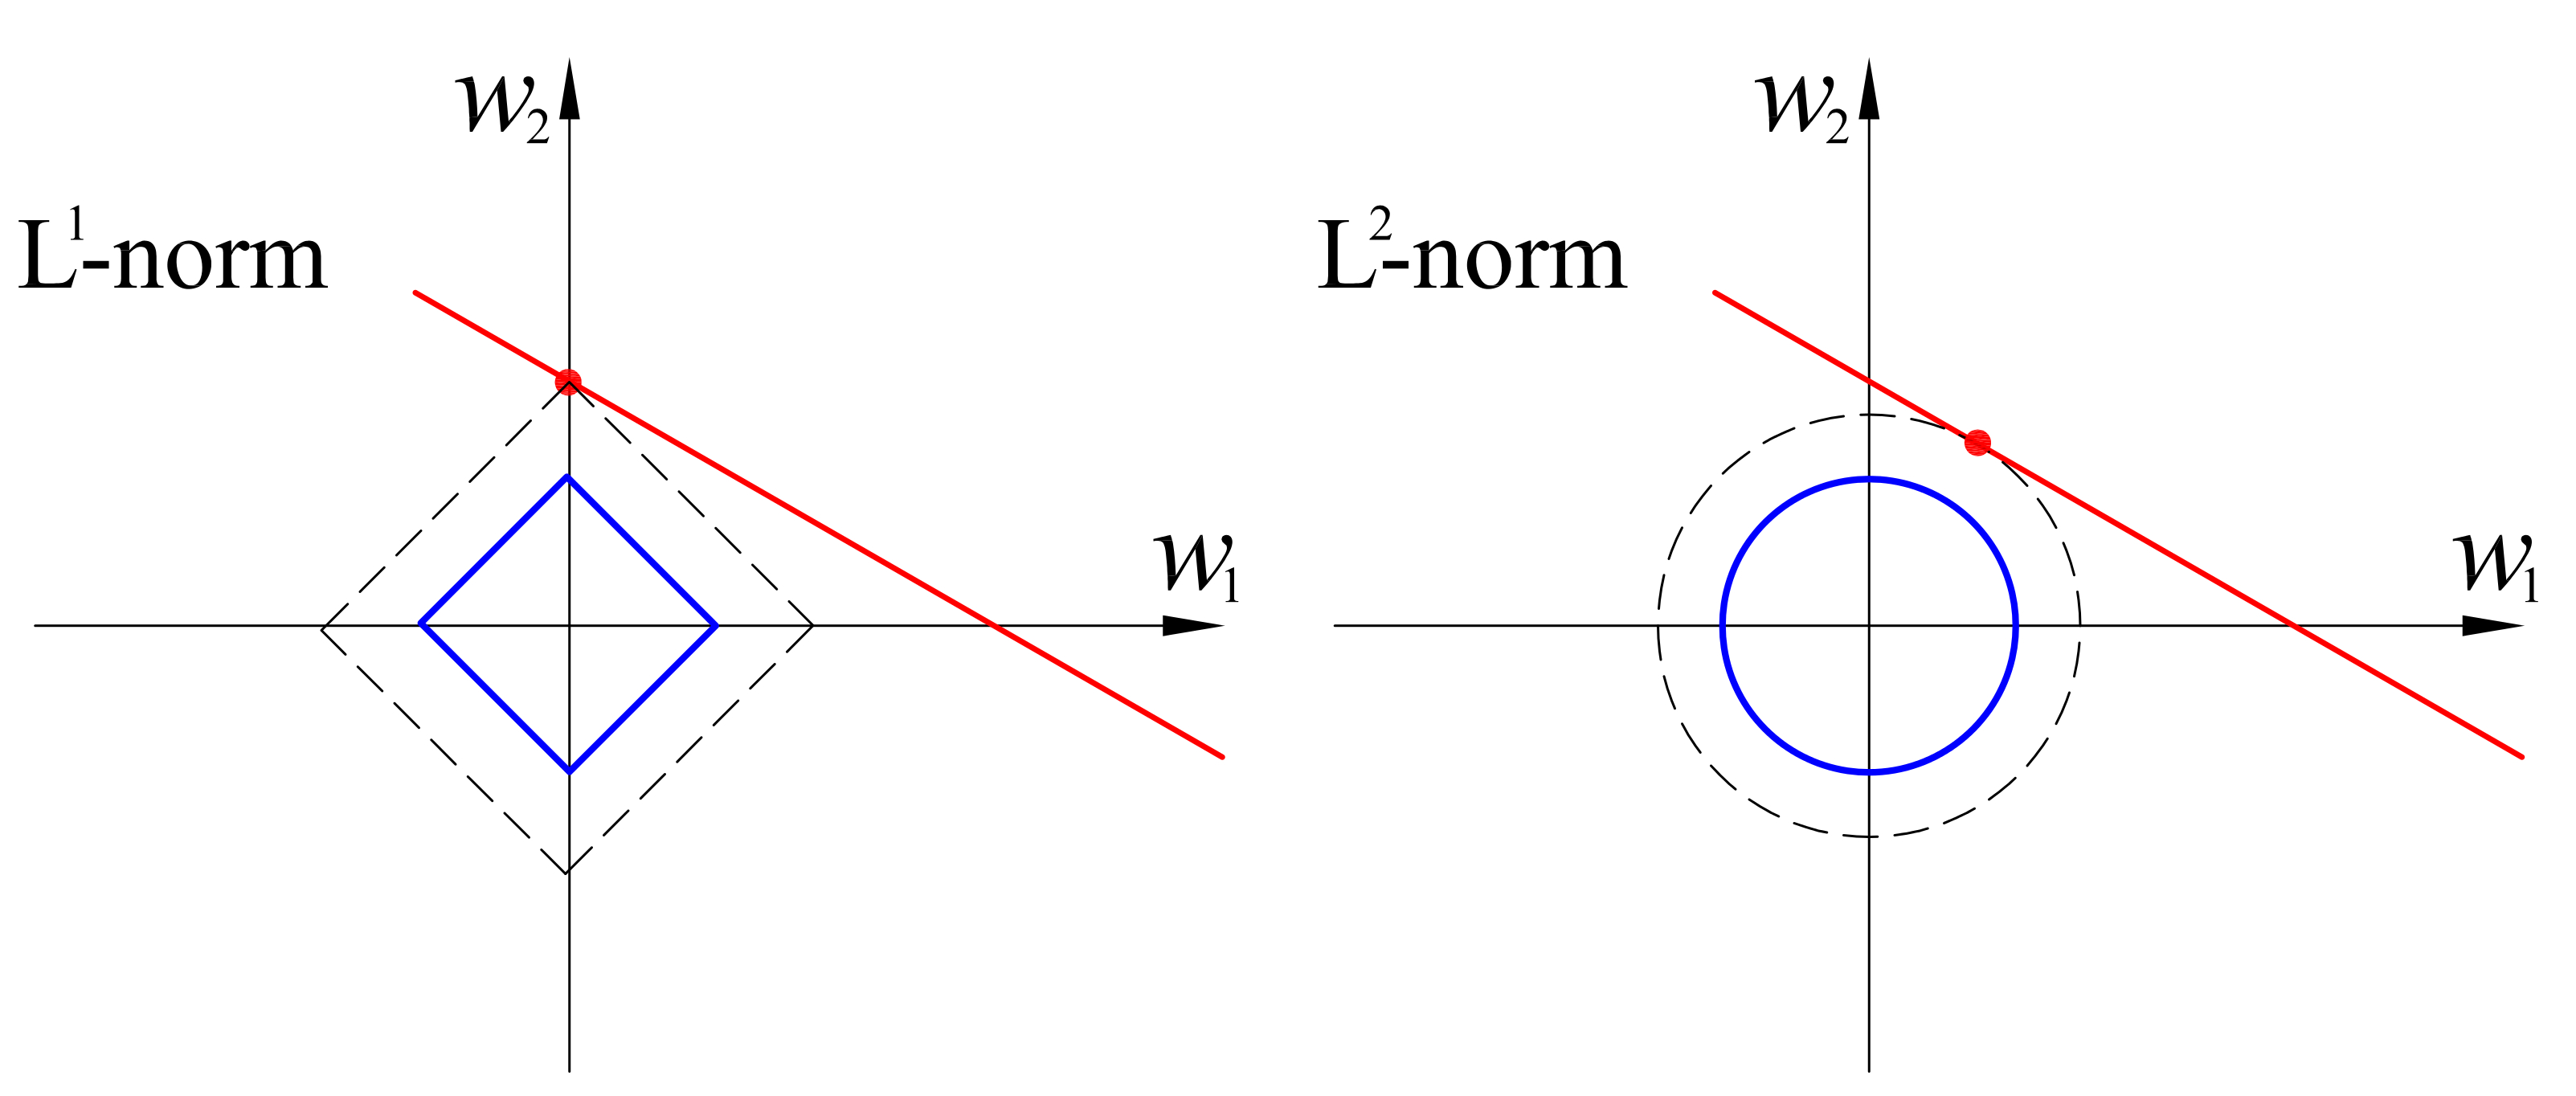
\includegraphics[width=0.5\textwidth]
        {share/shape.jpg}
    \end{figure}

    Finally, we \emph{cross-validate} the \emph{Lasso model} with \emph{k-fold cross-validation} using the \emph{glmnet library}. By using $k = 20$ and using \emph{M.S.E.} as the metric, we find the last plot in Figure~\ref{fig:lasso_ridge} which shows that the chosen features (the dotted interval) are those that produce the lowest M.S.E. Which are the 14 selected features. This is shown in the lines \texttt{96-97} of Listing~\ref{lst:script}. Lastly, we compare these results with those found with \emph{stepAIC}. Notice how the \emph{Lasso model} with \emph{k-fold C.V.} produced a much lower number of selected features, 14, while \emph{stepAIC()} produced a total of 64. \emph{Lasso} gives us less features.

    \newpage

    \begin{figure}[h!]
        \centering
        \caption{below are the relationships between the \emph{coefficients} and the \emph{$log(\lambda)$ penalty} for \emph{Ridge} and \emph{Lasso regression} (shown below in that exact order). Notice how \emph{Ridge} converges all of the \emph{coefficients simultaneously} while \emph{Lasso} does this step \emph{iteratively}, therefore, \emph{Lasso regression} should converge ``faster''. Finally, the bottom plot displays how a \emph{Lasso C.V.} relates to the increasing of \emph{penalty factor} of $log(\lambda)$.}
        \label{fig:lasso_ridge}
        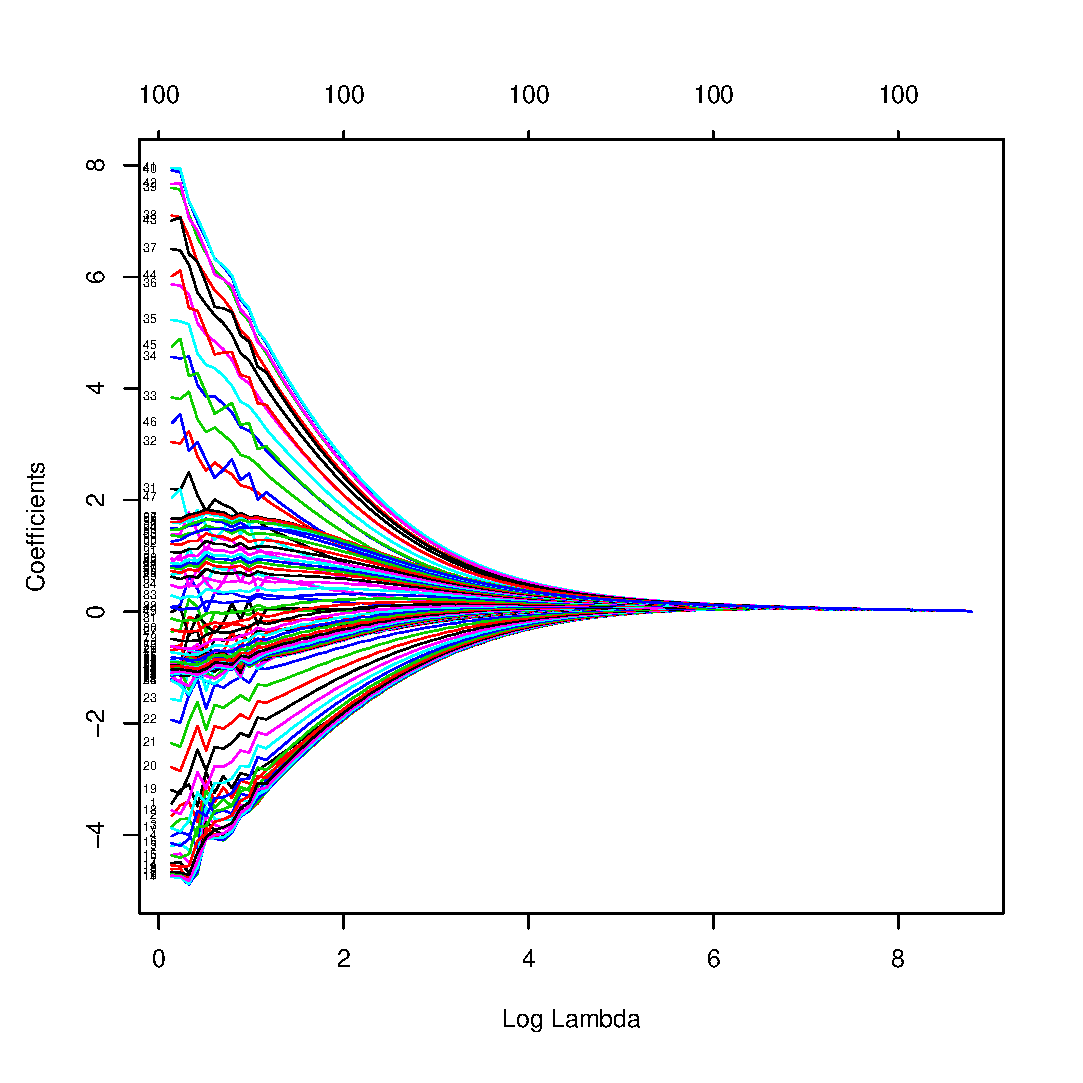
\includegraphics[width=0.35\textwidth]{share/ridge.eps}
        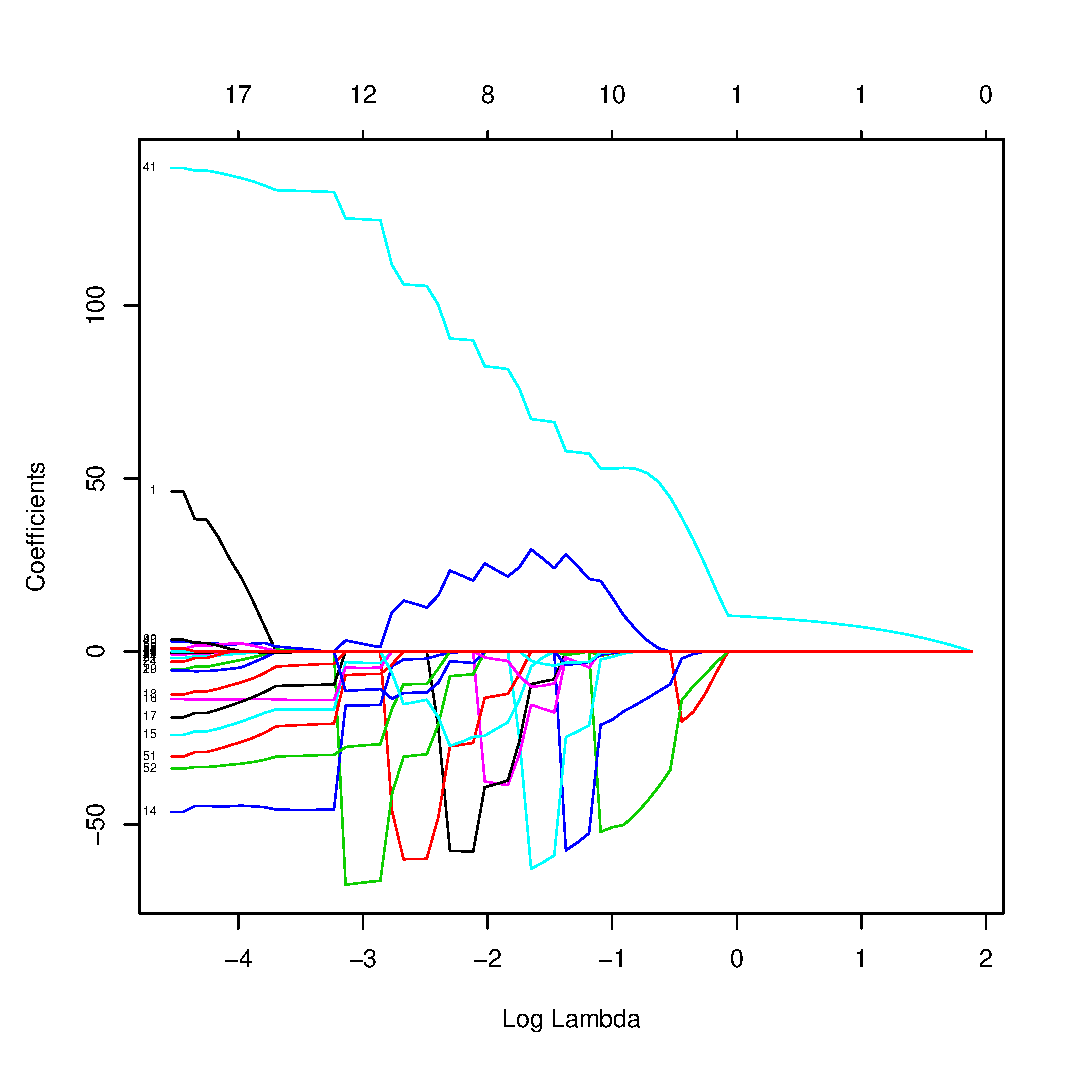
\includegraphics[width=0.35\textwidth]{share/lasso.eps}
        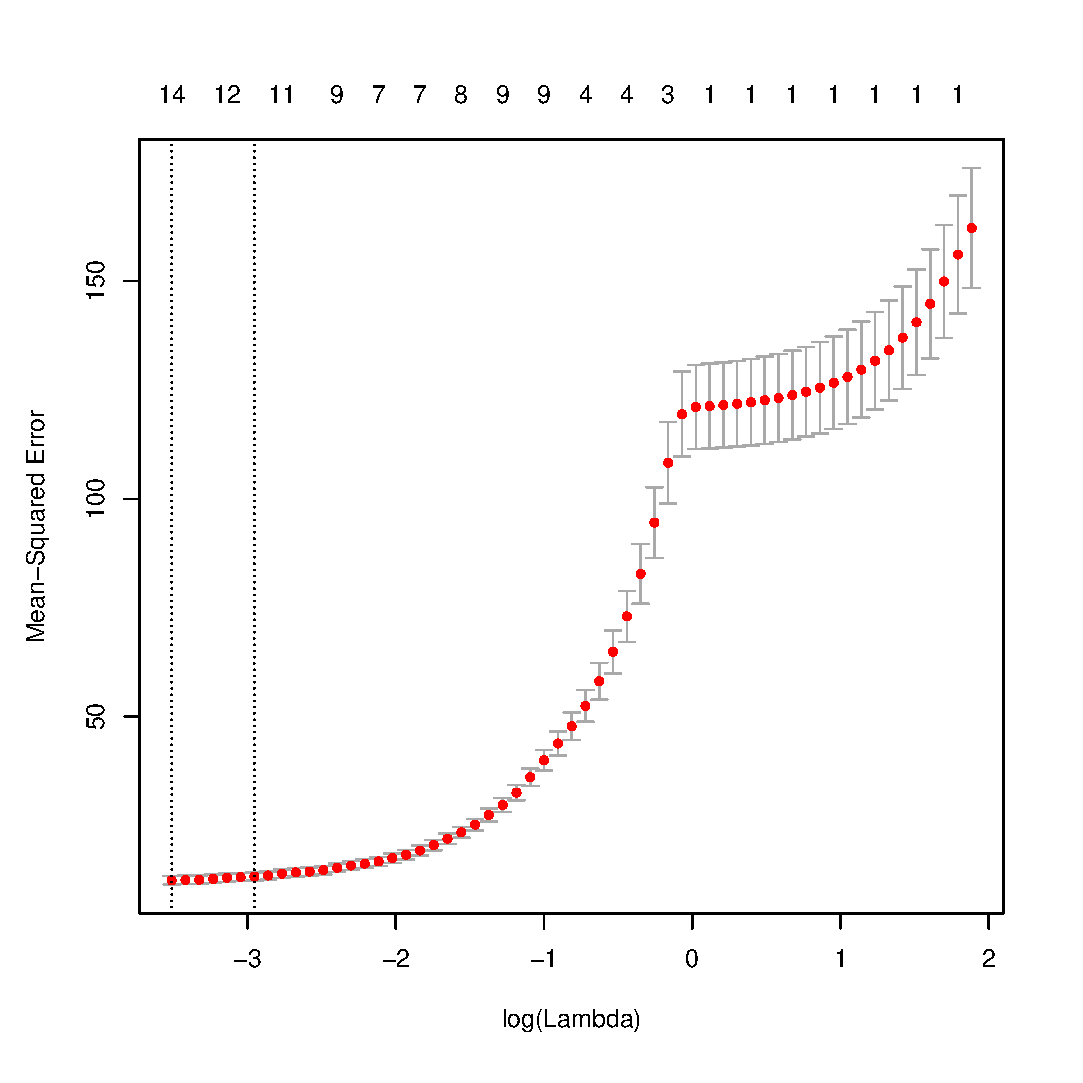
\includegraphics[width=0.35\textwidth]{share/kfold.eps}
    \end{figure}

    \clearpage \nocite{*}
    \bibliographystyle{alpha}
    \bibliography{report}

    \onecolumn \appendix
    \section*{Appendix}

    \lstinputlisting[caption={Estimation of the Linear Regression Model with a Hat Matrix},label={lst:linrhat}]{../assignment1/linrhat.r}
    \lstinputlisting[caption={Implementation of a K-Fold Cross-Validation Algorithm for $\mathcal{M}$},label={lst:kfoldcv}]{../assignment1/kfoldcv.r}
    \lstinputlisting[caption={Brute-Force Feature Selection to Find Lowest M.S.E. Subset},label={lst:featsel}]{../assignment1/featsel.r}
    \lstinputlisting[caption={Script for Assignment 2 on Linear Models, Ridge, Lasso and Cross-Validation},label={lst:script}]{../assignment2/script.r}

\end{document}
